%   % !TEX root = ../../VIII,3_Rahmen-TeX_8-1.tex
%  
%   Band VIII, 3		Rubrik STOSS
%
%   Signatur/Tex-Datei:	LH_35_09_21_007
%
%   RK-Nr. 	41205
%
%   \ref{\RK41205}
%
%   Überschrift: 	[Modus demonstrandi leges percussionis]
%   
%   Unterrubrik:			Unklar? Kinematik? Überblick?
%
%   edlabels:			0
%
%   Diagramme: 		7
%
%
%   NB: 						(Anmerkungen)					??
%
%
%
\selectlanguage{ngerman}
\frenchspacing
%
\begin{ledgroupsized}[r]{120mm}
\footnotesize
\pstart
\noindent\textbf{Überlieferung:}
\pend
\end{ledgroupsized}
%
\begin{ledgroupsized}[r]{114mm}
\footnotesize
\pstart \parindent -6mm
\makebox[6mm][l]{\textit{L}}%
Aufzeichnung:
LH~XXXV~9,~21 Bl.~7. 
Ein Blatt~8\textsuperscript{o};
Fragment eines Wasserzeichens;
Ränder beschnitten;
untere linke Ecke ohne Textverlust abgerissen.
Zwei Seiten;
Textfolge: Bl.~7~v\textsuperscript{o}, 7~r\textsuperscript{o}.
\pend
\end{ledgroupsized}
%
%
\count\Bfootins=1100%
\count\Afootins=1200%
\count\Cfootins=1100
\vspace{5mm}
\begin{ledgroup}
\footnotesize
\pstart
\noindent%
\textbf{Datierungsgründe:}%
\label{LH_35_09_21_007_Datierung}
Die titellose Aufzeichnung N.~\ref{RK41205} stellt in zwölf \glqq Propositionen\grqq\ eine Methode zum Nachweis der Gesetze des direkten zentralen Stoßes dar.
Diese beruht letztlich auf der Annahme, dass der Stoß zweier Körper, deren Geschwindigkeiten sich umgekehrt wie die Massen verhalten, dem Fall des Gleichgewichts einer Waage gleichgesetzt werden könne.
Die Aufzeichnung ist auf einem Träger verfasst, dessen Wasserzeichen für den Zeitraum 1680 bis 1685 mehrfach belegt ist.
Daraus ergibt sich die vorgeschlagene Datierung.
Zur Bekräftigung sei bemerkt, dass N.~\ref{RK41205} wichtige Ergebnisse voraussetzt, die Leibniz in seiner Untersuchung über die Stoßgesetze im Textkomplex \textit{De corporum concursu} (N.~\ref{dcc_00}) % , Anfang 1678
und insbesondere in der \textit{Scheda VIII} (N.~\ref{dcc_08}, Januar 1678) erreicht hat.
Das sind die quadratische Auffassung der \glqq kinetischen\grqq\ Kraft (N.~\ref{RK41205}, S.~\refpassage{LH_35_09_21_007v_par1-1}{LH_35_09_21_007v_par1-2},
\refpassage{LH_35_09_21_007r_par10-1}{LH_35_09_21_007r_par10-2}); %: Gleichgewicht ergebe sich beim Stoß, wenn die Wirkungen bzw. die Höhen, zu denen die Körper erhoben würden, sich umgekehrt wie die Massen der Körper verhielten
die Methode der \textit{compositio motuum} % \textendash\ die \glqq Schiff\grqq-Methode \textendash\ 
zur Berechnung der Stoßfälle, bei denen die Geschwindigkeiten sich nicht umgekehrt wie die Massen verhalten (ebd., S.~\refpassage{LH_35_09_21_007r_par11-1}{LH_35_09_21_007r_par11-2});
das Gesetz der Erhaltung der relativen Geschwindigkeit (ebd., S.~\refpassage{LH_35_09_21_007r_par12-1}
{LH_35_09_21_007r_par12-2}).
\pend%
%
%\pstart%
%Das Wasserzeichen (Hirsch ohne Kugel mit Buchstaben \glqq IH\grqq, LEd-WZ 803027) ist lt.\ Datenbanken für den \textit{Zeitraum 1680\textendash1685} mehrfach belegt. (Eine Vorgängerversion, 803003, ist 1677\textendash1682 belegt).%
%\pend
%%
%\pstart
%%
%Prop.~10 (Bl.~7~r\textsuperscript{o}) verwendet den Begriff \textit{vis} für $mv$. Dort heißt es: \glqq Itaque hic contingit vires esse aequales, quoad conflictum, si sint reciproce pondera ut celeritates.\grqq. D.h. vis\textsubscript{A} = vis\textsubscript{B}  genau dann, wenn $\dfrac{m_A}{m_B} = \dfrac{v_B}{v_A}$; dies ist aber äquivalent zu $m_A v_A = m_B v_B$.\\
%Dieser Umstand würde für eine Datierung \textit{vor dem \textit{DCC} (Januar 1678)} sprechen, wenn man ihn sehr ernst nimmt (d.h. \textit{wenn} man annimmt, dass Leibniz ab der Scheda Octava des \textit{DCC} den Begriff vis \textit{nur noch und ausnahmslos} für $mv^2$ verwendet).%
%\pend
%%
%\pstart
%%
%Prop.~3 unterscheidet zwischen \textit{conatus (aut impetus)} \textit{vivus} und \textit{mortuus}, denen sowohl die mathematische Dimensionalität (endliche vs. infinitesimale Größe) als auch die physische Interpretation (a \textit{primum} se restituentis impulsu vs. ex motu \textit{aliquamdiu} accelerato) zukommen, die aus der Physik der mittleren Jahre bekannt sind. Ab wann ist diese Unterscheidung belegt? Könnte dieser Umstand evtl. für eine \textit{etwas spätere Datierung} sprechen?
%\pend %
%%
%\pstart
%\textbf{Unterrubrik:} Kinematik? Oder Überblicksdarstellungen?
%\pend 
%
\end{ledgroup}
%
\selectlanguage{latin}
\frenchspacing
\count\Bfootins=1100%
\count\Afootins=1200%
\count\Cfootins=1100
% \newpage%
\vspace{8mm}
\pstart%
\normalsize%
\noindent%
%
\lbrack7~v\textsuperscript{o}\rbrack\ %%%% Bl. 7v
%
Inveni modum demonstrandi leges percussionis.%
\protect\index{Sachverzeichnis}{lex percussionis}%
\protect\index{Sachverzeichnis}{percussio}%
\protect\index{Sachverzeichnis}{modus demonstrandi}
Atque ita ordior a notis.%
\protect\index{Sachverzeichnis}{notum}%
\pend%
\pstart%
1. Si
%
\edtext{duo pondera}{%
\lemma{duo}\Bfootnote{%
\textit{(1)}~corpora
\textit{(2)}~pondera%
~\textit{L}}}
%
\textit{A} et \textit{B}
incumbunt%
\protect\index{Sachverzeichnis}{pondus incumbens}
brachiis oppositis ejusdem librae \textit{C},%
\protect\index{Sachverzeichnis}{brachium librae}
ita ut conatus descendendi%
\protect\index{Sachverzeichnis}{conatus descendendi}
sint reciproce
%
\edtext{ut pondera,%
\protect\index{Sachverzeichnis}{conatus reciproce ut pondera}
erunt}{%
\lemma{ut}\Bfootnote{%
\textit{(1)}~corpora, er
\textit{(2)}~pondera, erunt%
~\textit{L}}}
%
in aequilibrio.%
\protect\index{Sachverzeichnis}{aequilibrium}
Ita enim et
%
\edlabel{LH_35_09_21_007v_par1-1}%
\edtext{effectus%
\protect\index{Sachverzeichnis}{effectus factus ex altitudine}%
\protect\index{Sachverzeichnis}{effectus in pondus}%
\protect\index{Sachverzeichnis}{effectus aequalis}%
\lbrack,\rbrack\
facti scilicet ex altitudinibus in pondera%
\lbrack,\rbrack\
utrinque aequales orirentur,
alterutro vincente.%
\edlabel{LH_35_09_21_007v_par1-2}
%\pend%
\newline%
%
%\pstart%
\indent%
2. Idque fiet sive}{%
\lemma{effectus}\Bfootnote{%
\textit{(1)}~. 2. Idque continget sive
\textit{(2)}~facti scilicet % ex altitudinibus in pondera utrinque aequales orirentur,
\lbrack...\rbrack\ alterutro vincente. \lbrack/\rbrack\ 2.
\textit{(a)}~Idem est
\textit{(b)}~Idque fiet sive%
~\textit{L}}}
%
conatus%
\protect\index{Sachverzeichnis}{conatus descendendi}
vel velocitates%
\protect\index{Sachverzeichnis}{velocitas descendendi}
%
\edtext{descendendi differant}{%
\lemma{descendendi}\Bfootnote{%
\textit{(1)}~sint diversi
\textit{(2)}~differant%
~\textit{L}}}
%
ob distantiam majorem minoremve%
\protect\index{Sachverzeichnis}{distantia a centro librae}
a centro librae%
\protect\index{Sachverzeichnis}{centrum librae}%
\protect\index{Sachverzeichnis}{libra}
%
\edtext{(\protect\vphantom)%
ut in communi mechanica%
\protect\index{Sachverzeichnis}{mechanica communis}%
\protect\vphantom();}{%
\lemma{(\protect\vphantom)ut}\Bfootnote{%
\hspace{-0,5mm}in communi mechanica\protect\vphantom()
\textit{erg.~L}}}
%
sive aliunde,
si brachia librae \textit{AC}, \textit{BC}%
\protect\index{Sachverzeichnis}{brachium librae}%
\protect\index{Sachverzeichnis}{libra}
sint aequalia\lbrack,\rbrack\
corpora autem \textit{A} et \textit{B}
%
\edtext{vel alieno impulsu%
\protect\index{Sachverzeichnis}{impulsus alienus}
vel}{%
\lemma{vel}\Bfootnote{%
\textit{(1)}~aliunde vel
\textit{(2)}~alieno impulsu vel%
~\textit{L}}}
%
jam concepto conatu%
\protect\index{Sachverzeichnis}{conatus conceptus}
diversas velocitates habeant.%
\protect\index{Sachverzeichnis}{velocitas descendendi}
\pend%
%
%
\vspace{1.5em}%
\centerline{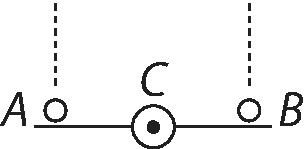
\includegraphics[width=0.18\textwidth]{gesamttex/edit_VIII,3/images/LH_35_09_21_007_d1_007v.pdf}}
\vspace{0.5em}
\centerline{\lbrack\textit{Fig.~1}\rbrack}
%
%
%
\pstart%
3.
%
\edlabel{LH_35_09_21_007v_par3-1}
\edtext{Idque sive illi conatus%
\protect\index{Sachverzeichnis}{conatus mortuus}
aut impetus%
\protect\index{Sachverzeichnis}{impetus mortuus}
sint mortui}{%
\lemma{Idque}\Bfootnote{%
\textit{(1)}~si est cona
\textit{(2)}~sive illi conatus
\textbar~aut impetus \textit{erg.}~%
\textbar\ sint mortui%
~\textit{L}}}
%
seu infinite parvi paulatim crescentes,%
\protect\index{Sachverzeichnis}{conatus infinite parvus}%
\protect\index{Sachverzeichnis}{conatus paulatim crescentes}
si verbi gratia a gravitate propria%,%
\protect\index{Sachverzeichnis}{gravitas propria}
vel elaterii%,%
\protect\index{Sachverzeichnis}{elaterium se restituens}
nunc primum se restituentis impulsu%
\protect\index{Sachverzeichnis}{impulsus elaterii}
oriantur;
%
sive sint vivi,%
\protect\index{Sachverzeichnis}{impetus vivus}%
\protect\index{Sachverzeichnis}{conatus vivus}
concepti scilicet ex motu aliquamdiu accelerato,%
\protect\index{Sachverzeichnis}{conatus conceptus}%
\protect\index{Sachverzeichnis}{conatus ex motu accelerato}%
\protect\index{Sachverzeichnis}{motus acceleratus}
ut si duo corpora \textit{A} et \textit{B}
%
ex diversis altitudinibus%
\protect\index{Sachverzeichnis}{altitudo incidentiae}
in bilancem%
\protect\index{Sachverzeichnis}{bilanx}
incidant,%
\protect\index{Sachverzeichnis}{corpus incidens in bilancem}
aequali quidem distantia%
\protect\index{Sachverzeichnis}{distantia a centro librae}
%
\edtext{a centro,}{%
\lemma{a}\Bfootnote{%
\hspace{-0,5mm}centro
\textit{erg.~L}}}
%
sed velocitatibus inaequalibus % ,
quae sint reciproce ut pondera%
\protect\index{Sachverzeichnis}{velocitas inaequalis}%
\protect\index{Sachverzeichnis}{velocitates ponderibus reciproce proportionales}%
\lbrack,\rbrack\
ponamusque libram plane esse rigidam et inflexilem,%
\protect\index{Sachverzeichnis}{libra rigida}%
\protect\index{Sachverzeichnis}{libra inflexilis}
sese mutuo impedient.%
\edlabel{LH_35_09_21_007v_par3-2}
\pend%
%
\pstart%
4.
Itaque in hoc ipso casu%
\lbrack,\rbrack\
si Elastica%
\protect\index{Sachverzeichnis}{corpus elasticum}
esse ponantur%
\lbrack,\rbrack\
ambo%
\protect\index{Sachverzeichnis}{corpus reflexum}
%
\edtext{\lbrack reflectentur\rbrack}{%
\lemma{reflectentur}\Bfootnote{%
\textit{erg. Hrsg.}}}
%
ea celeritate%
\protect\index{Sachverzeichnis}{celeritas reflexionis}
qua venerunt.
\pend%
%
%
\vspace{1.0em}
\centerline{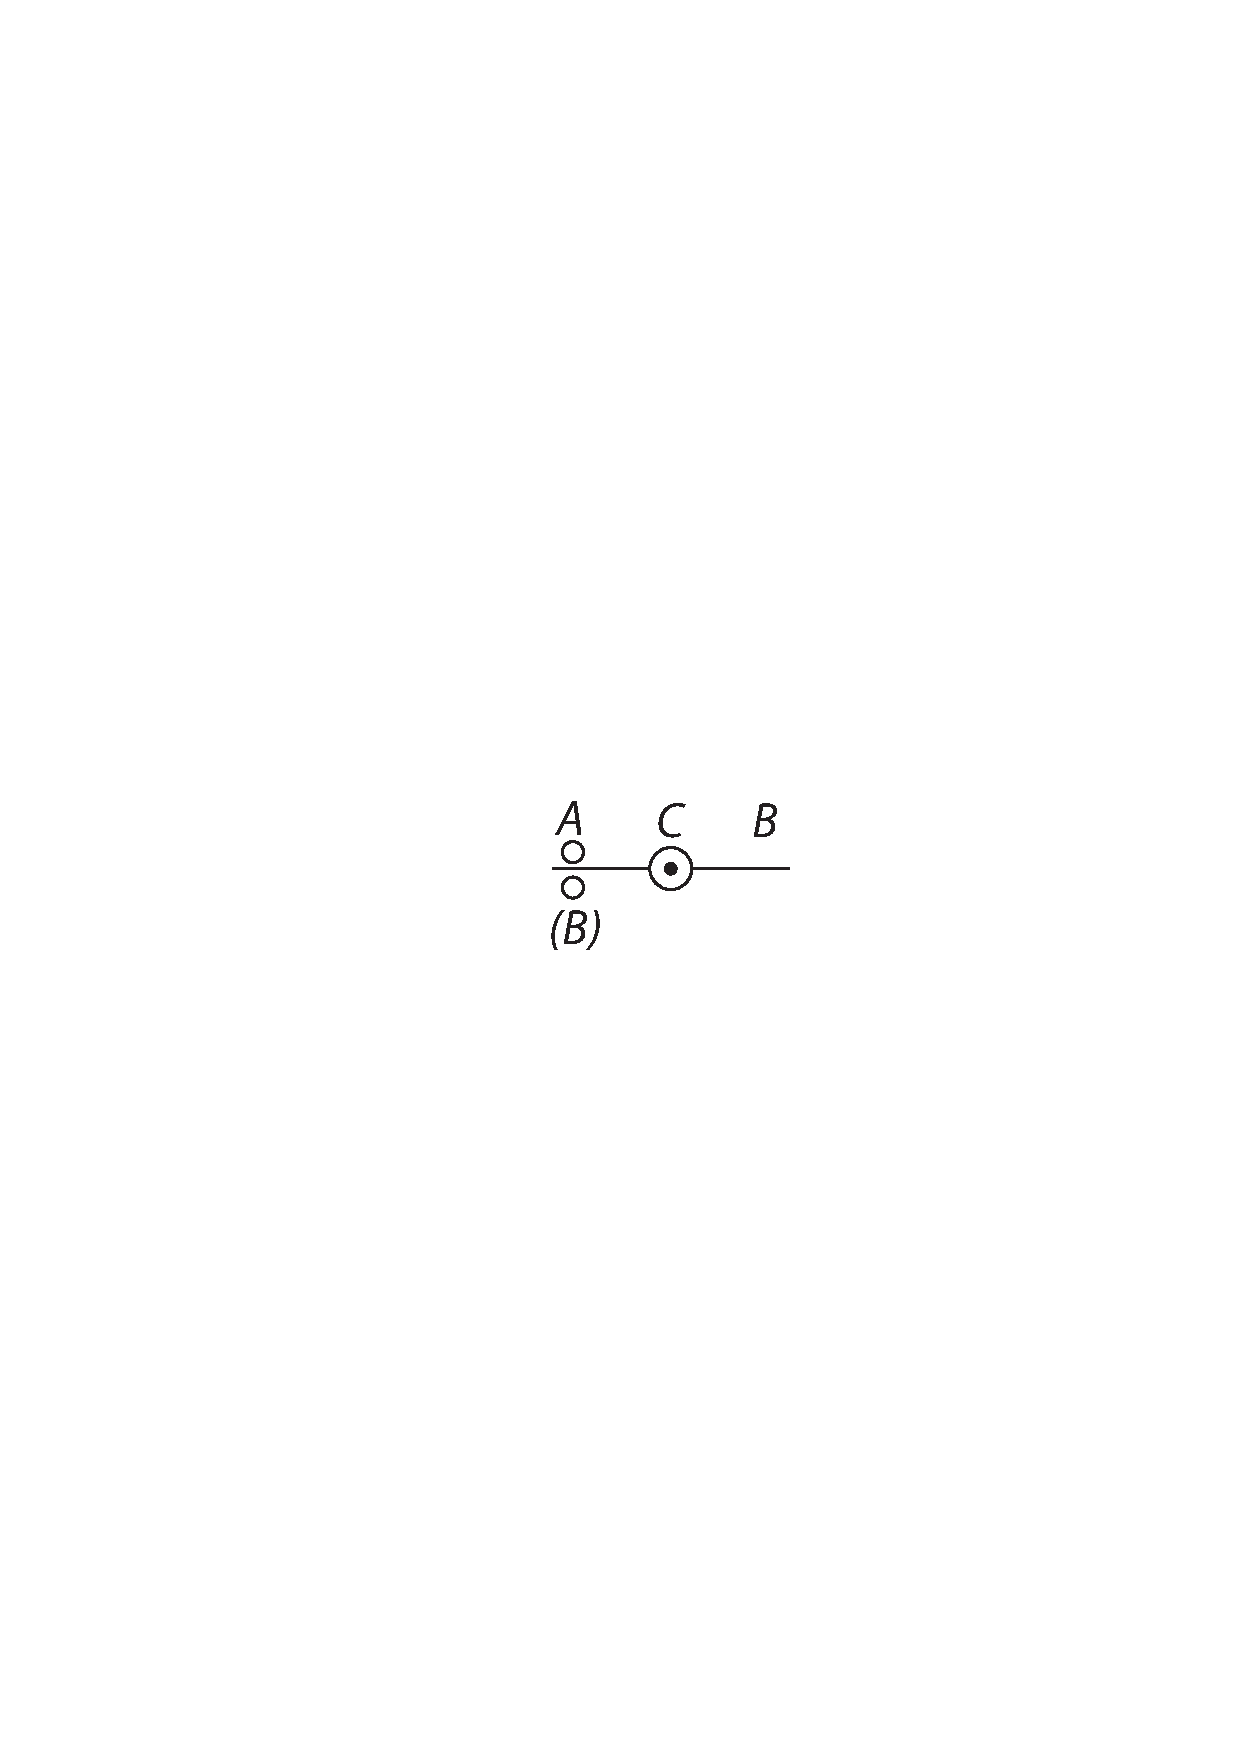
\includegraphics[width=0.16\textwidth]{gesamttex/edit_VIII,3/images/LH_35_09_21_007_d2_007v.pdf}}%
\vspace{0.3em}
\centerline{\lbrack\textit{Fig.~2}\rbrack}
\vspace{1.0em}
\pstart%
%
%
5.
Idem est
si ambo corpora%
\protect\index{Sachverzeichnis}{corpus incidens in libram}
non tendant in easdem partes in
%
\edtext{oppositis librae brachiis%
\protect\index{Sachverzeichnis}{brachium librae}%
\protect\index{Sachverzeichnis}{libra}%
}{%
\lemma{oppositis}\Bfootnote{%
\textit{(1)}~partibus
\textit{(2)}~librae brachiis%
~\textit{L}}}
%
in \textit{A} et \textit{B},
sed tendant in oppositas
%
\edtext{partes in eodem}{%
\lemma{partes}\Bfootnote{%
\hspace{-0,5mm}in
\textit{(1)}~iisdem librae brachiis
\textit{(2)}~eodem librae brachio%
~\textit{L}}}
%
librae brachio,%
\protect\index{Sachverzeichnis}{brachium librae}%
\protect\index{Sachverzeichnis}{libra}
ita ut \textit{A} et \textit{(B)} sibi occurrant
in eadem distantia a \textit{C},%
\protect\index{Sachverzeichnis}{distantia a centro librae}
%
\edtext{unum descendens%
\protect\index{Sachverzeichnis}{corpus descendens}
alterum ascendens.%
\protect\index{Sachverzeichnis}{corpus ascendens}%
}{%
\lemma{unum}\Bfootnote{%
\textit{(1)}~ascendens
\textit{(2)}~descendens alterum ascendens.%
~\textit{L}}}
%
%
\edtext{Si fuisset opus
potuissemus prius \textit{A} et \textit{(B)} admovere
in diversis distantiis%
\protect\index{Sachverzeichnis}{distantia a centro librae}
ejusdem brachii,%
\protect\index{Sachverzeichnis}{brachium librae}
et tandem venire ad eandem.%
}{%
\lemma{Si}\Bfootnote{%
fuisset \lbrack...\rbrack\ ad eandem.
\textit{erg.~L}}}
%
\pend%
%
\pstart%
6.
Et cum hoc modo nihil referat
quanta sit longitudo ipsius \textit{CA} vel \textit{C(B)},
patet \textit{CA} vel \textit{CB} plane posse omitti
idemque fore
si \textit{A} et \textit{(B)} sibi hoc modo%
\lbrack,\rbrack\
interjecto tantum aliquo rigido \textit{LM},%
\protect\index{Sachverzeichnis}{rigidum}
occurrant.
%
%
\pend%
\vspace{1.0em}
\centerline{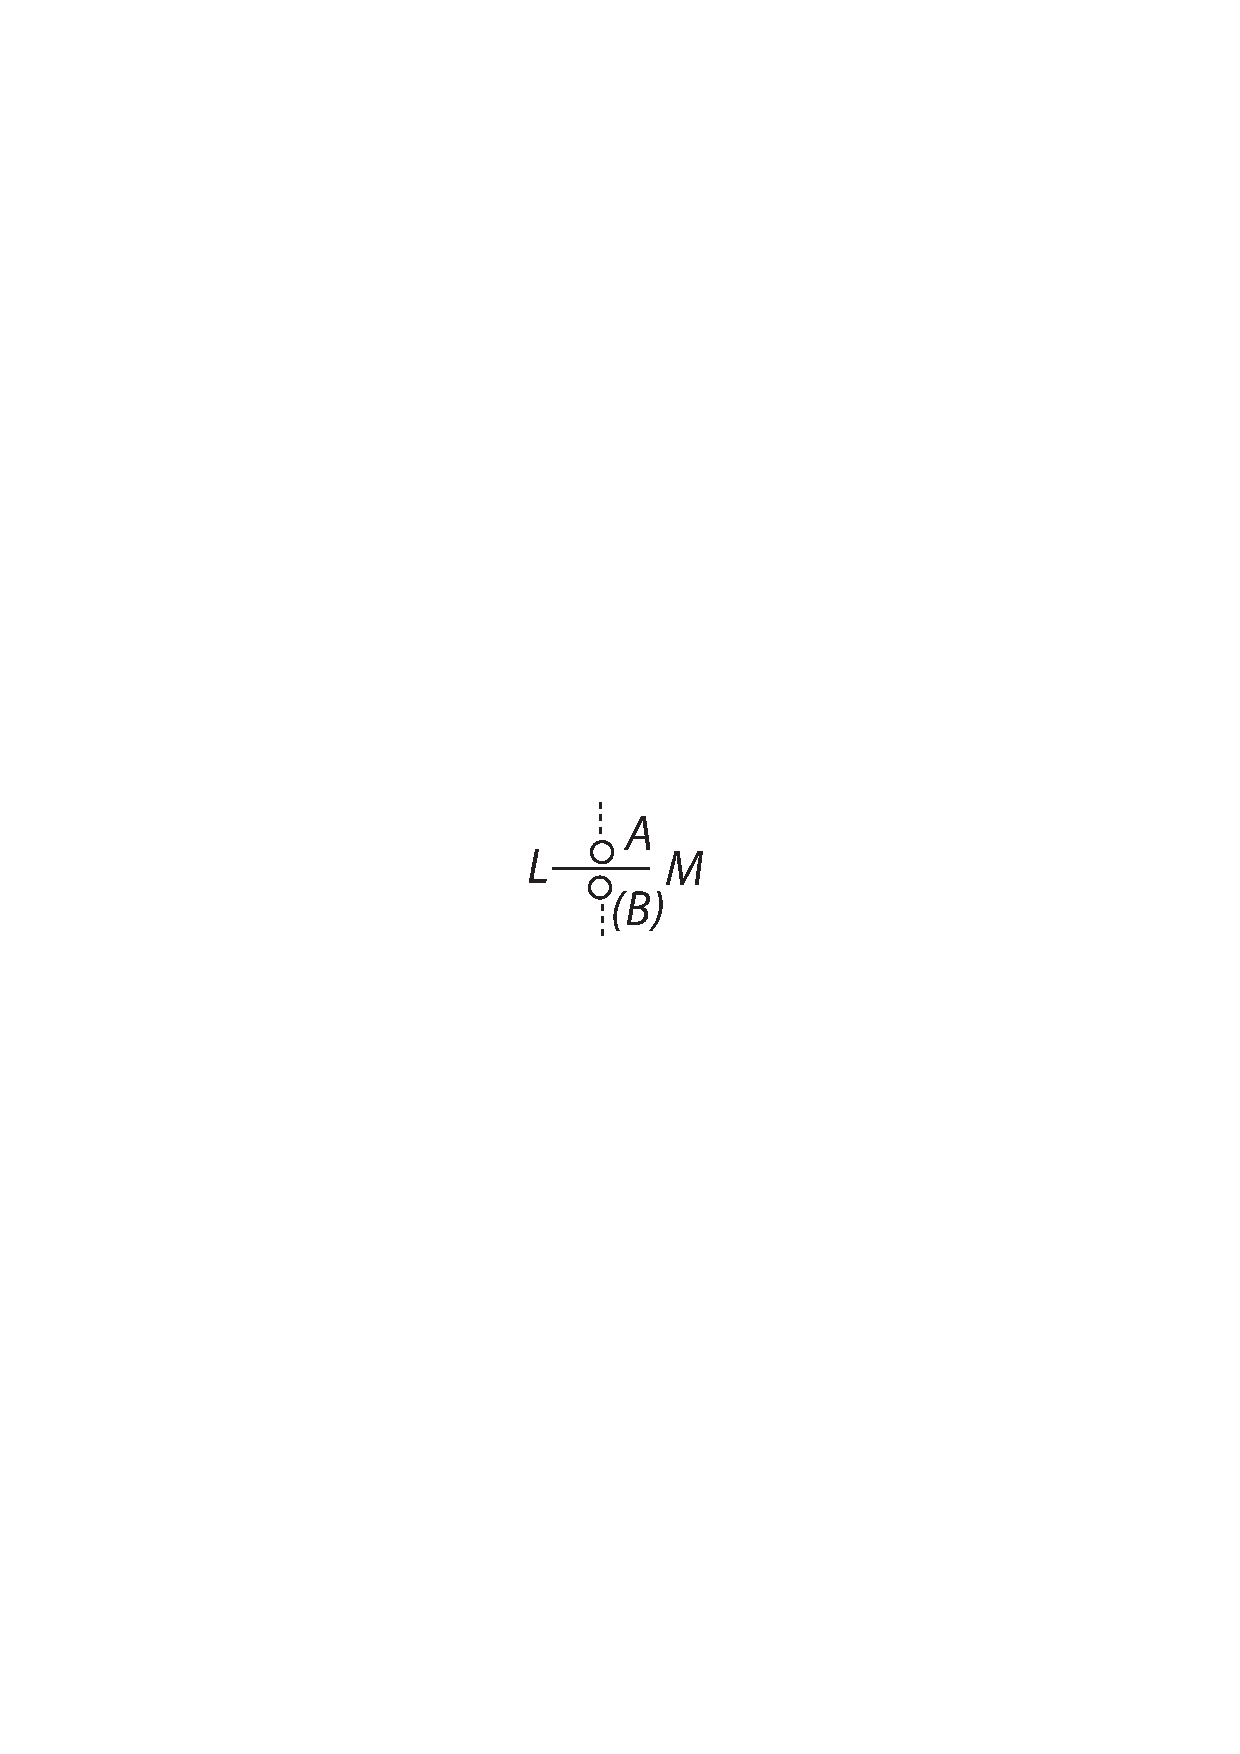
\includegraphics[width=0.12\textwidth]{gesamttex/edit_VIII,3/images/LH_35_09_21_007_d3_007v.pdf}}
\vspace{0.3em}
\centerline{\lbrack\textit{Fig.~3}\rbrack}
\vspace{1.0em}
%
%
\pstart%
7.
Immo quia rigidum illud potest esse utcunque tenue,%
\protect\index{Sachverzeichnis}{rigidum}%
\protect\index{Sachverzeichnis}{tenue}
poterit esse
%
\edtext{infinitesimae magnitudinis,%
\protect\index{Sachverzeichnis}{magnitudo infinitesima}
seu nullius,%
\protect\index{Sachverzeichnis}{magnitudo nulla}%
}{%
\lemma{infinitesimae}\Bfootnote{%
\textit{(1)}~hoc est
\textit{(2)}~magnitudinis, seu nullius,%
~\textit{L}}}
%
adeoque plane omitti,%
\protect\index{Sachverzeichnis}{magnitudo omissa}
ac proinde
si duo corpora \textit{A} et \textit{B} sibi
%
\edtext{directe}{%
\lemma{directe}\Bfootnote{%
\textit{erg.~L}}}
%
occurrant%
\protect\index{Sachverzeichnis}{corpora sibi occurrentia}
unum descendendo,%
\protect\index{Sachverzeichnis}{corpus descendens}
alterum ascendendo,%
\protect\index{Sachverzeichnis}{corpus ascendens}
sintque velocitates ponderibus reciproce proportionales,%
\protect\index{Sachverzeichnis}{velocitates ponderibus reciproce proportionales}
sibi mutuo progressum impedient%
\protect\index{Sachverzeichnis}{progressus mutuo impeditus}%
\lbrack;\rbrack\
%
\edtext{et si}{%
\lemma{et}\Bfootnote{%
\textit{(1)}~si elast
\textit{(2)}~si
\textit{(3)}~si%
~\textit{L}}}
%
sunt elastica%
\protect\index{Sachverzeichnis}{corpus elasticum}
reflectentur%
\protect\index{Sachverzeichnis}{corpus reflexum}
qua venerunt celeritate.%
\protect\index{Sachverzeichnis}{celeritas reflexionis}
%
\lbrack7~r\textsuperscript{o}\rbrack\ %%%% Bl. 7r
%
\pend%
%
\vspace{1.0em}
\centerline{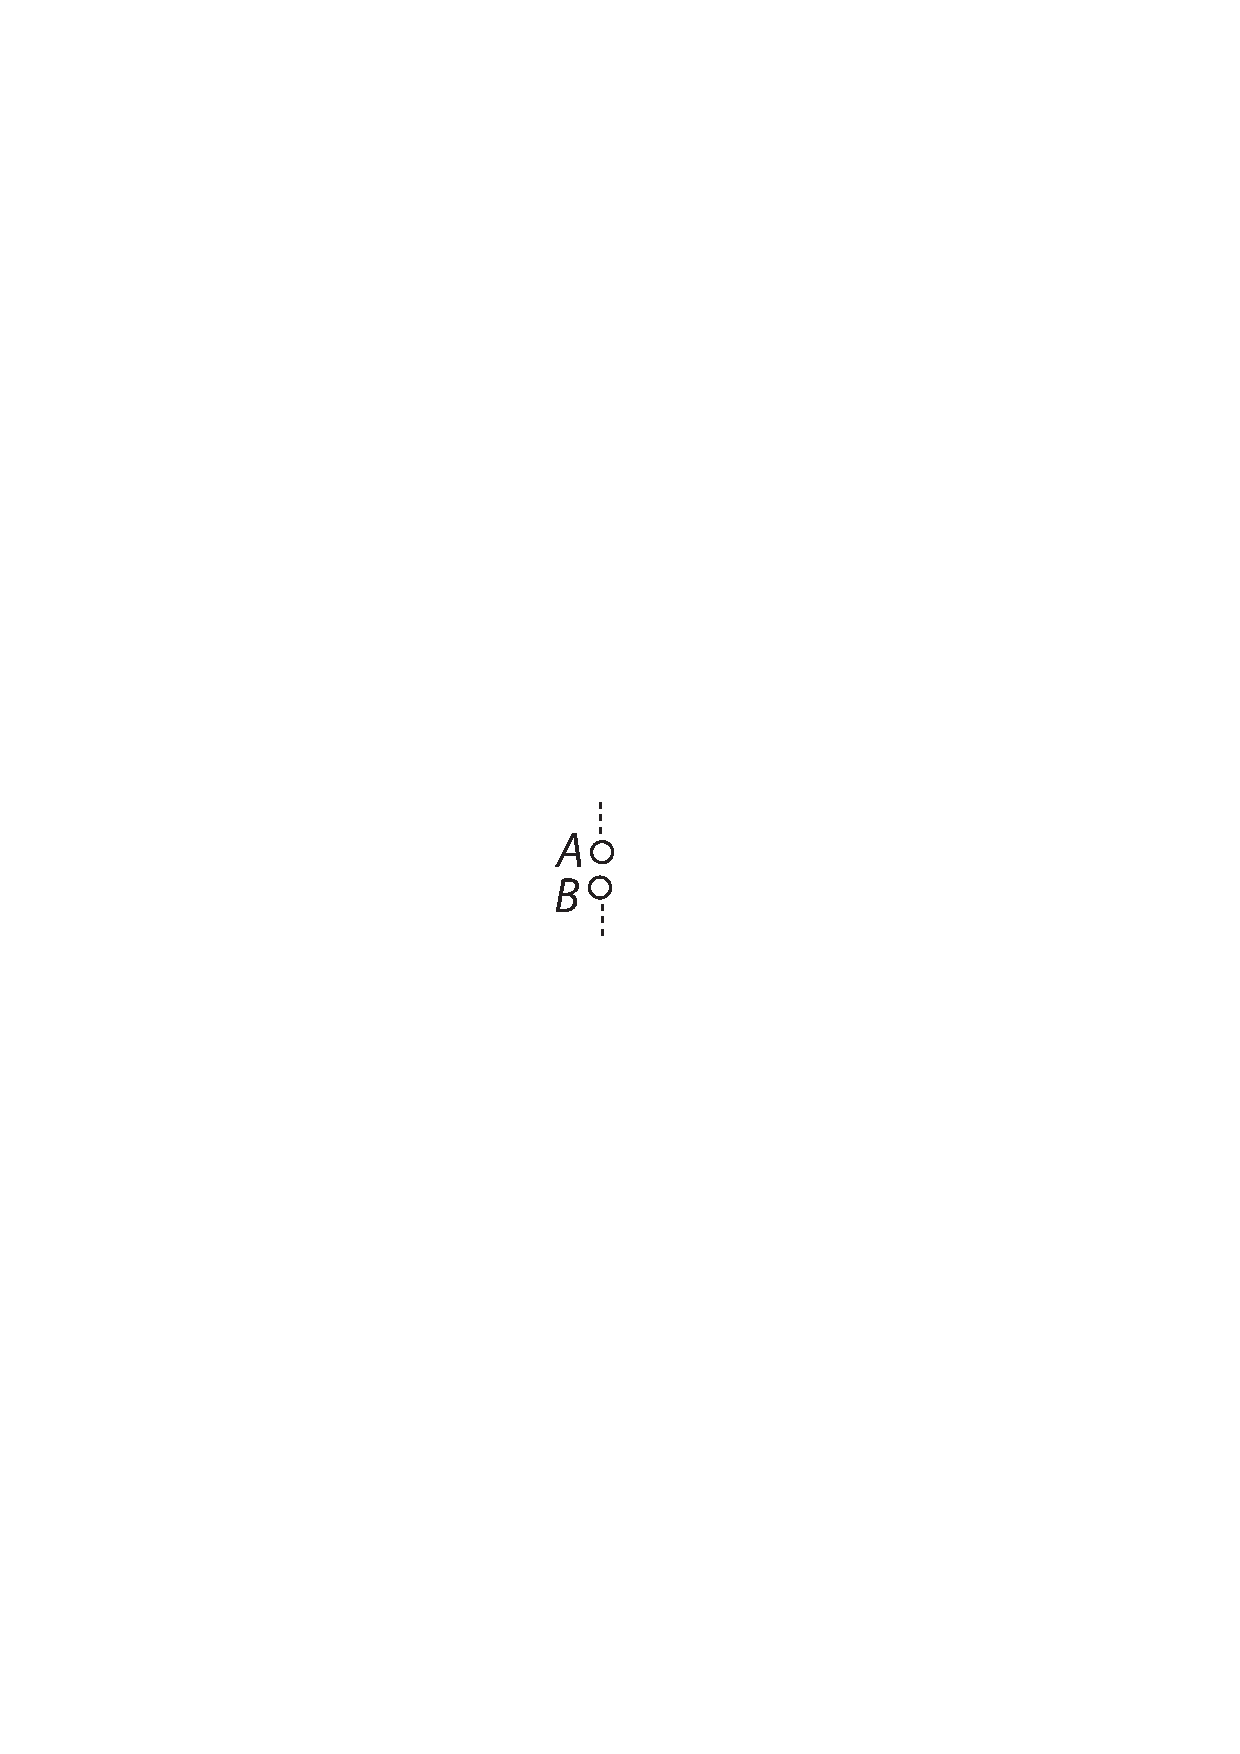
\includegraphics[width=0.06\textwidth]{gesamttex/edit_VIII,3/images/LH_35_09_21_007_d4_007v.pdf}}
\vspace{0.2em}
\centerline{\lbrack\textit{Fig.~4}\rbrack}
\vspace{1.0em}
\pstart%
8.
Idem erit
etsi linea descensus%
\protect\index{Sachverzeichnis}{linea ascensus}%
\protect\index{Sachverzeichnis}{ascensus}
ascensusque%
\protect\index{Sachverzeichnis}{linea descensus}%
\protect\index{Sachverzeichnis}{descensus}
non sit perpendicularis%
\protect\index{Sachverzeichnis}{linea perpendicularis}
sed inclinata.%
\protect\index{Sachverzeichnis}{linea inclinata}%
\pend%
%
%
\vspace{1.0em}
\centerline{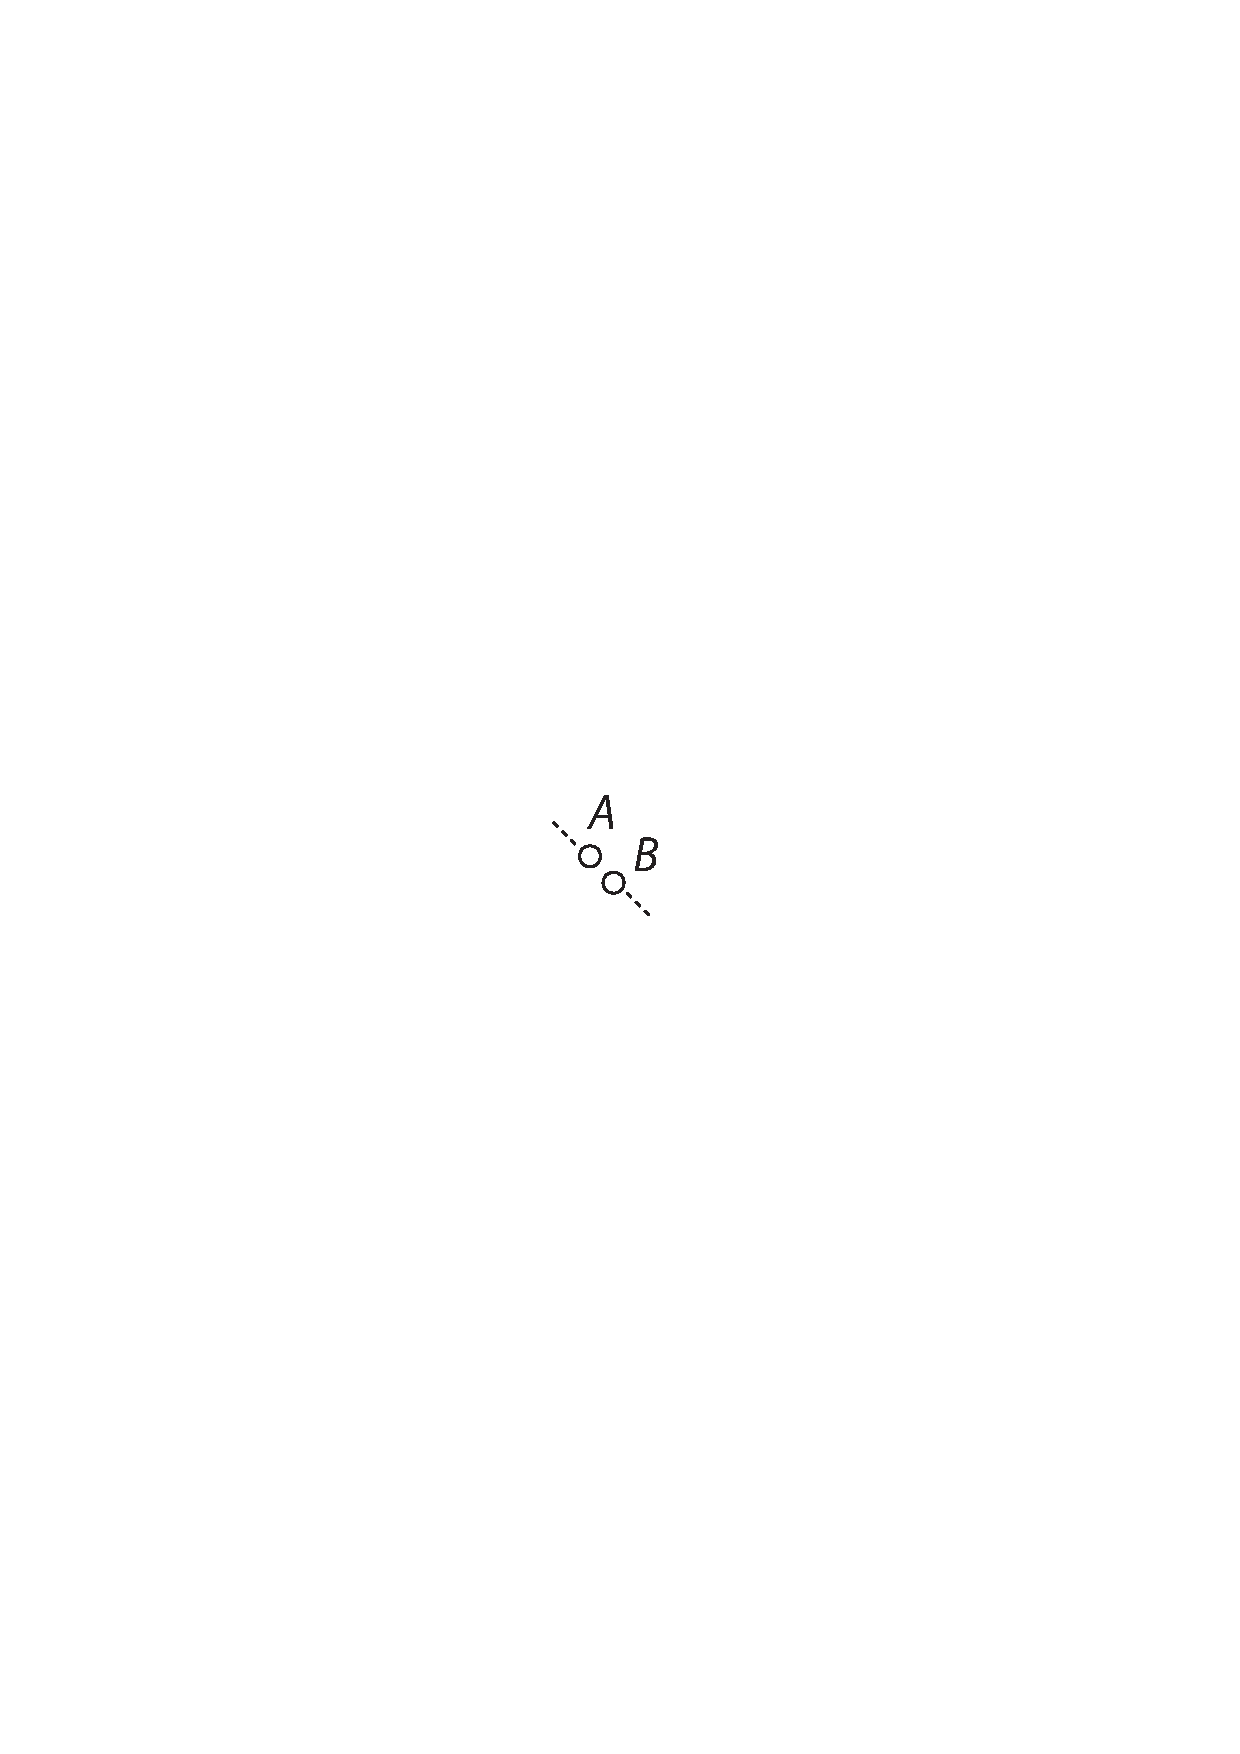
\includegraphics[width=0.08\textwidth]{gesamttex/edit_VIII,3/images/LH_35_09_21_007_d5_007r.pdf}}
\vspace{0.2em}
\centerline{\lbrack\textit{Fig.~5}\rbrack}
\vspace{1.0em}
%
%
\pstart%
9.
Quare idem quoque erit
si inclinatio%
\protect\index{Sachverzeichnis}{inclinatio quantacunque}
sit quantacunque,
adeoque tandem maxima,%
\protect\index{Sachverzeichnis}{inclinatio maxima}
ita ut linea motus%
\protect\index{Sachverzeichnis}{linea motus}
ab horizontali%
\protect\index{Sachverzeichnis}{linea horizontalis}
differat minus differentia qualibet data,%
\protect\index{Sachverzeichnis}{differentia quaelibet data}
adeoque haberi possit horizontalis.%
\protect\index{Sachverzeichnis}{linea horizontalis}
Itaque si
%
\edtext{duo pondera}{%
\lemma{duo}\Bfootnote{%
\textit{(1)}~corpora
\textit{(2)}~pondera%
~\textit{L}}}
%
\textit{A} et \textit{B} in linea horizonti parallela,
vel alia quacunque sibi occurrant directe,%
\protect\index{Sachverzeichnis}{corpora sibi occurrentia}
ita ut velocitates eorum 
%
sint ponderibus reciproce proportionales,%
\protect\index{Sachverzeichnis}{velocitates ponderibus reciproce proportionales}
mutuo sibi progressum impedient;%
\protect\index{Sachverzeichnis}{progressus mutuo impeditus}
ac si elastica sint,%
\protect\index{Sachverzeichnis}{corpus elasticum}
ea qua venerunt celeritate reflectentur.%
\protect\index{Sachverzeichnis}{corpus reflexum}
\pend%
%
%
\vspace{1.0em}
\centerline{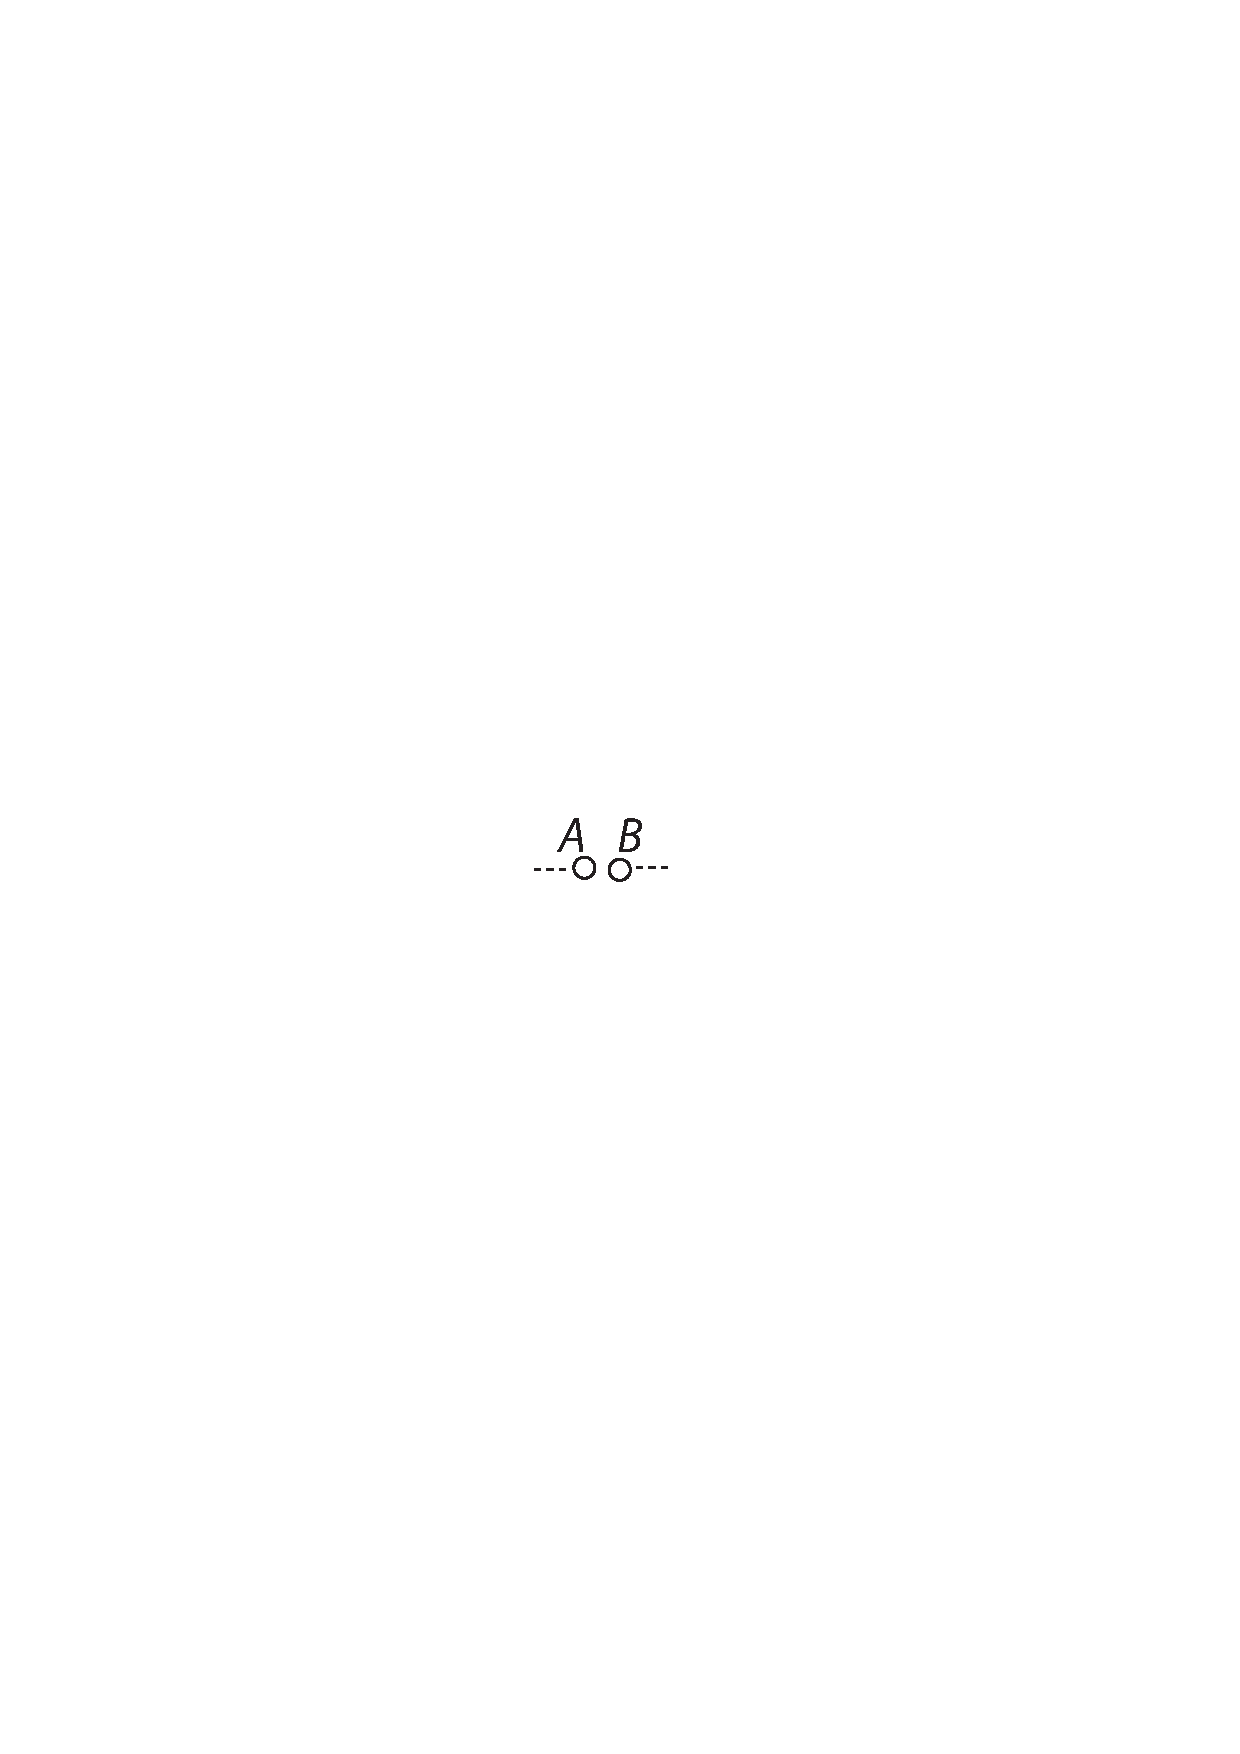
\includegraphics[width=0.1\textwidth]{gesamttex/edit_VIII,3/images/LH_35_09_21_007_d6_007r.pdf}}
\vspace{0.3em}
\centerline{\lbrack\textit{Fig.~6}\rbrack}
\vspace{1.0em}
%
%
\pstart%
10.
Brevius ad idem potuissemus pervenire
demonstrando immediate propositionem 7%
\protect\index{Sachverzeichnis}{propositio}
%
ex principio communi,%
\protect\index{Sachverzeichnis}{principium commune}
eo ipso scilicet unde demonstratur 
%
prop. 1,%
\protect\index{Sachverzeichnis}{propositio}
nempe quod occurrentibus sibi directe duobus corporibus%
\protect\index{Sachverzeichnis}{corpora sibi occurrentia}
extra omnem libram,%
\protect\index{Sachverzeichnis}{libra}
ita ut
%
\edtext{unum conetur attollere vel deprimere alterum,%
\protect\index{Sachverzeichnis}{corpus alterum attollens}%
\protect\index{Sachverzeichnis}{corpus alterum deprimens}%
\protect\index{Sachverzeichnis}{corpus conans}%
}{%
\lemma{unum}\Bfootnote{%
\textit{(1)}~descendat, alte
\textit{(2)}~conetur attollere vel deprimere alterum,%
~\textit{L}}}
%
\edlabel{LH_35_09_21_007r_par10-1}%
aequilibrium sit,%
\protect\index{Sachverzeichnis}{aequilibrium}
si effectus%
\protect\index{Sachverzeichnis}{effectus seu altitudo}%
\protect\index{Sachverzeichnis}{altitudo seu effectus}
seu
%
\edtext{altitudines attollendi%
\protect\index{Sachverzeichnis}{altitudo attollendi}}{%
\lemma{altitudines}\Bfootnote{%
\textit{(1)}~ad quas
\textit{(2)}~attollendi%
~\textit{L}}}
%
forent corporibus reciproce proportionales;%
\protect\index{Sachverzeichnis}{effectus corporibus reciproce proportionales}%
\protect\index{Sachverzeichnis}{altitudines corporibus reciproce proportionales}
forent autem eae hic%
\lbrack,\rbrack\
saltem in primo ascendendi conatu,%
\protect\index{Sachverzeichnis}{conatus ascendendi}%
\protect\index{Sachverzeichnis}{conatus primus}
ut celeritates.
%
Itaque hic contingit
vires esse aequales,
quoad conflictum,%
\protect\index{Sachverzeichnis}{vires aequales quoad conflictum}%
\protect\index{Sachverzeichnis}{conflictus}
%
si sint reciproce pondera ut celeritates.%
\edlabel{LH_35_09_21_007r_par10-2}%
\protect\index{Sachverzeichnis}{celeritates corporibus reciproce proportionales}
Idem ergo est secundum prop.%
\protect\index{Sachverzeichnis}{propositio}
8 et 9
%
\edtext{licet lineae}{%
\lemma{licet}\Bfootnote{%
\textit{(1)}~pondera
\textit{(2)}~lineae%
~\textit{L}}}
%
\edtext{\lbrack descensuum\rbrack%
\protect\index{Sachverzeichnis}{linea descensus}%
\protect\index{Sachverzeichnis}{descensus}%
}{%
\lemma{descensum}\Bfootnote{%
\textit{L~ändert Hrsg.}}}
%
aut ascensuum%
\protect\index{Sachverzeichnis}{linea ascensus}%
\protect\index{Sachverzeichnis}{ascensus}
sint utcunque inclinatae%
\protect\index{Sachverzeichnis}{linea inclinata}
donec fiat plane horizontalis.%
\protect\index{Sachverzeichnis}{linea horizontalis}
\pend%
%
%
\newpage%\vspace{0.5em}
\centerline{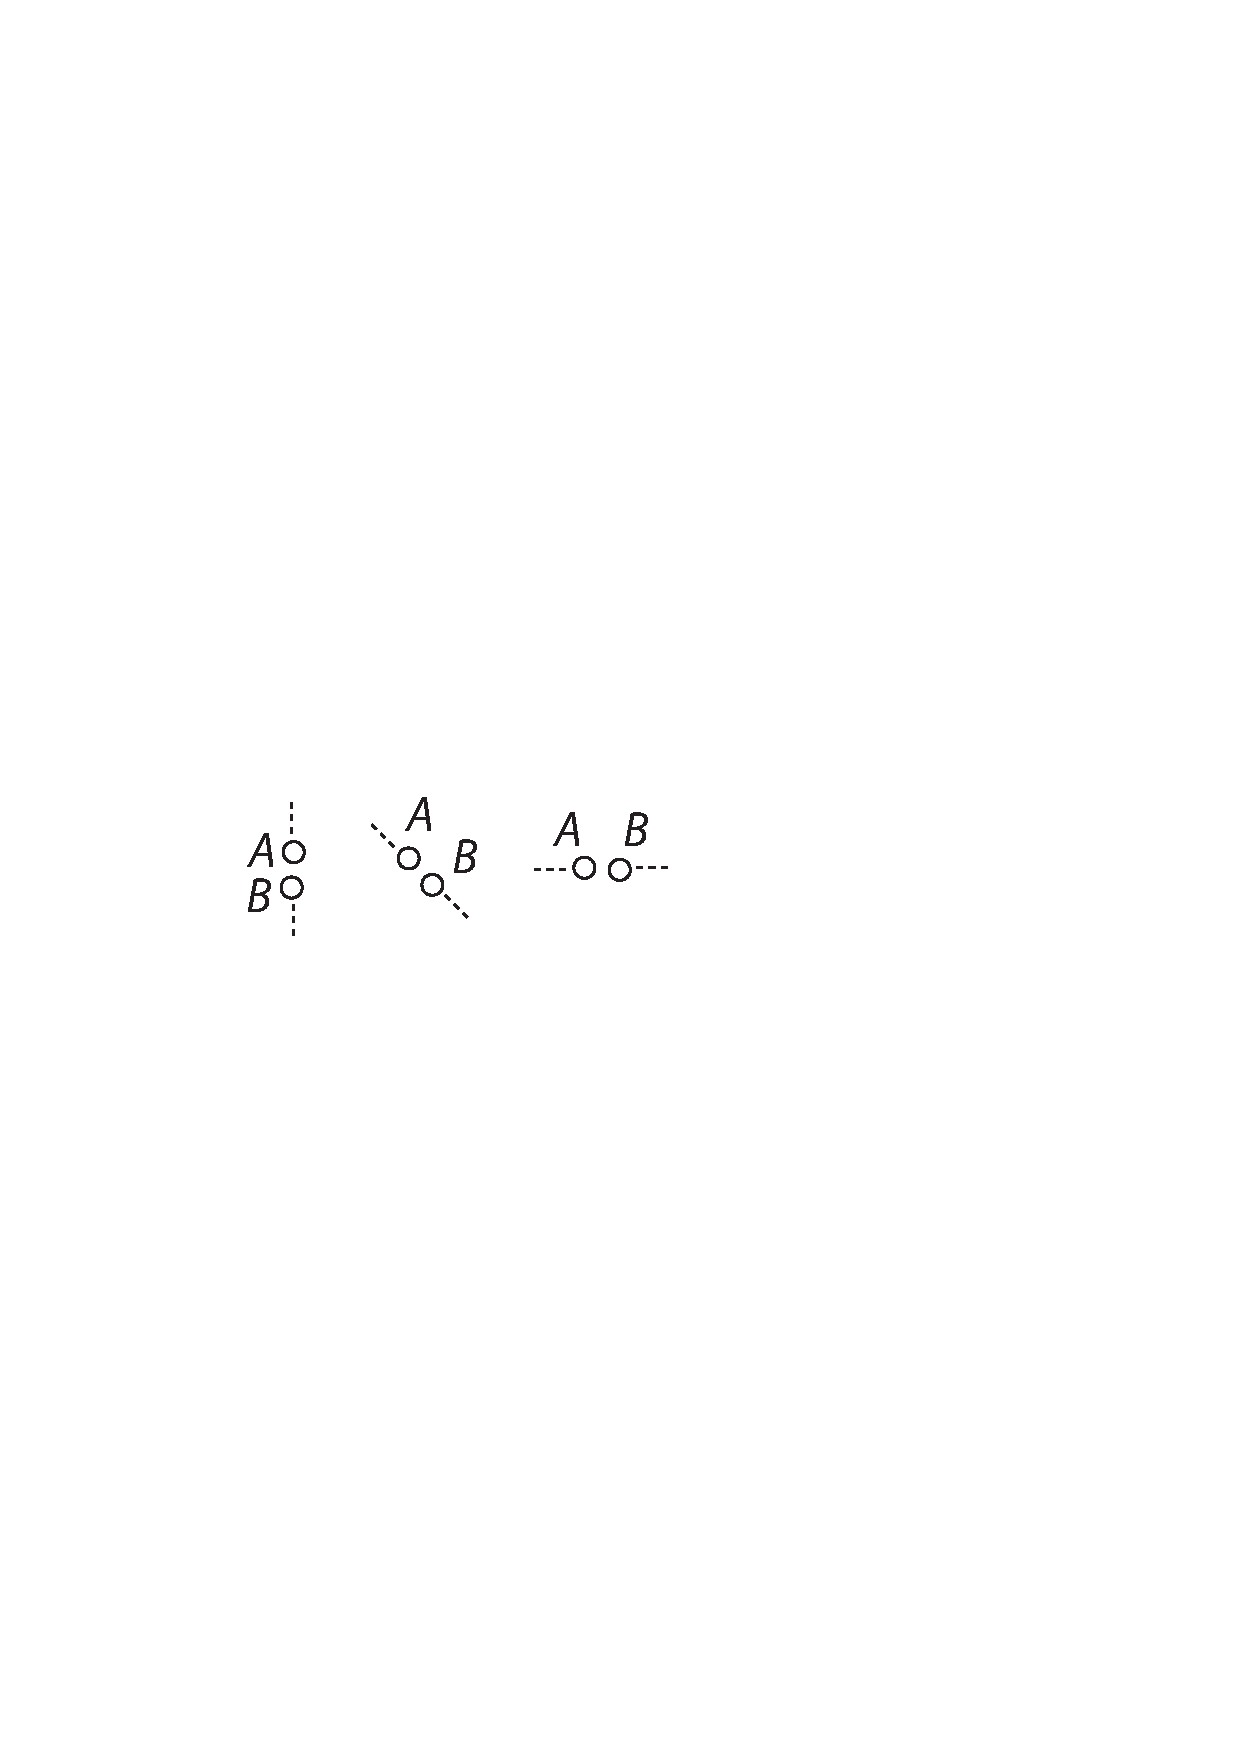
\includegraphics[width=0.26\textwidth]{gesamttex/edit_VIII,3/images/LH_35_09_21_007_d7u8u9_007r.pdf}}
\vspace{0.3em}
\centerline{\lbrack\textit{Fig.~7}\rbrack}
\vspace{1.0em}
%
%
\pstart
11.
\edlabel{LH_35_09_21_007r_par11-1}%
Hinc jam porro demonstratur
quid fiat in aliis casibus%
\protect\index{Sachverzeichnis}{casus alius}
cum corpora duo in plano Horizontali sibi occurrunt%
\protect\index{Sachverzeichnis}{corpora sibi occurrentia}%
\protect\index{Sachverzeichnis}{planum horizontale}%
\protect\index{Sachverzeichnis}{occursus in plano horizontali}
aliis celeritatibus quam
quae sint reciproce proportionales%
\protect\index{Sachverzeichnis}{celeritates aliae quam ponderibus reciproce proportionales}
%
\edtext{ponderibus%
\lbrack,\rbrack\
ponendo}{%
\lemma{ponderibus}\Bfootnote{%
\textit{(1)}~cum enim ictus\protect\index{Sachverzeichnis}{ictus}
\textit{(2)}~fingen
\textit{(3)}~ponendo%
~\textit{L}}}
%
quasi ambo moverentur in navi communi%,%
\protect\index{Sachverzeichnis}{navis communis}%
\protect\index{Sachverzeichnis}{corpus movens in navi}%
\protect\index{Sachverzeichnis}{motus in navi communi}
in qua ipsa sibi occurrerent%
\protect\index{Sachverzeichnis}{occursus in navi}%
\protect\index{Sachverzeichnis}{corpora sibi occurrentia in navi}
celeritatibus % ,
%
quae sint magnitudinibus reciproce proportionales,%
\protect\index{Sachverzeichnis}{celeritates ponderibus reciproce proportionales}
reliquam diversitatem%
\protect\index{Sachverzeichnis}{diversitas reliqua}
exhibendo per motum communem%
\protect\index{Sachverzeichnis}{motus communis cum navi}%
\protect\index{Sachverzeichnis}{diversitas exhibita per motum communem}
%
\edtext{\lbrack quem\rbrack}{%
\lemma{quam}%
\Bfootnote{%
\textit{L~ändert Hrsg.}}}
%
habent cum navi.%
\protect\index{Sachverzeichnis}{navis}%
\edlabel{LH_35_09_21_007r_par11-2}
\pend%
%
\pstart%
12.
\edlabel{LH_35_09_21_007r_par12-1}%
Idem et ex eo demonstrari potest,
quod ictus%
\protect\index{Sachverzeichnis}{ictus}
est idem seu percussio%
\protect\index{Sachverzeichnis}{percussio}
duorum corporum,
quando eadem est celeritas appropinquandi,%
\protect\index{Sachverzeichnis}{celeritas appropinquandi}
%
cuicunque demum eorum competat quies%
\protect\index{Sachverzeichnis}{quies aut motus}
aut motus.%
\protect\index{Sachverzeichnis}{motus aut quies}%
\edlabel{LH_35_09_21_007r_par12-2}
%
\edtext{\lbrack Tanta}{%
\lemma{\lbrack Tanta}\Cfootnote{Die eckige Klammer stammt von Leibniz.}}
%
enim vi resistit corpus%
\protect\index{Sachverzeichnis}{vis corporis quiescentis resistentis}%
\protect\index{Sachverzeichnis}{corpus quiescens resistens}%
\protect\index{Sachverzeichnis}{resistentia corporis quiescentis}
%
\edtext{quiescens ei
quod aliquam ipsi vim%
\protect\index{Sachverzeichnis}{vis accipienda}
daturum est,
quanta est vis%
\protect\index{Sachverzeichnis}{vis accipienda}
quam accipere debet.%
}{%
\lemma{quiescens}\Bfootnote{%
\textit{(1)}~\textbar~aequali \textit{erg.}~%
\textbar\ quod dato motu impellere conatur, quantam vim haberet, si jam eum motum accepisset
\textit{(2)}~ei quod aliquam ipsi
\textit{(a)}~celeritatem
\textit{(b)}~vim daturum % est, quanta est vis quam 
\lbrack...\rbrack\ accipere debet.%
~\textit{L}}}
%
Quod tamen
%
\edtext{ultimum}{%
\lemma{ultimum}\Bfootnote{%
\textit{erg.~L}}}
%
considerandum est paulo accuratius,
ut accurata habeatur
%
\edtext{enuntiatio.%
\protect\index{Sachverzeichnis}{enuntiatio accurata}\rbrack}{%
\lemma{enuntiatio.\rbrack}\Cfootnote{Die eckige Klammer stammt von Leibniz.}}
%
\pend
%
\pstart%
Videndum et an Elastra%
\protect\index{Sachverzeichnis}{elastrum}
diversa,
v.\,g. aeres diverse compressi%
\protect\index{Sachverzeichnis}{aer compressus}
celeritate diversa restitutionem%
\protect\index{Sachverzeichnis}{restitutio}%
\protect\index{Sachverzeichnis}{celeritas restitutionis}
incipiant.
\pend
\count\Bfootins=1200%
\count\Afootins=1200%
\count\Cfootins=1200
%
%
%%%% Ende des Textes auf Bl. 7r.